\documentclass[conference]{IEEEtran}
% \IEEEoverridecommandlockouts
% The preceding line is only needed to identify funding in the first footnote. If that is unneeded, please comment it out.
\usepackage{cite}
\usepackage{amsmath,amssymb,amsfonts}
\usepackage{algorithmic}
\usepackage{graphicx}
\usepackage{array}
\usepackage{textcomp}
\usepackage{xcolor}
\usepackage{url}
\def\BibTeX{{\rm B\kern-.05em{\sc i\kern-.025em b}\kern-.08em
    T\kern-.1667em\lower.7ex\hbox{E}\kern-.125emX}}
    
\makeatletter
\newcommand{\linebreakand}{%
  \end{@IEEEauthorhalign}
  \hfill\mbox{}\par
  \mbox{}\hfill\begin{@IEEEauthorhalign}
}
\makeatother

\begin{document}

\title{Using an Artificial Neural Network to Evaluate Chess Positions}

\author{
\IEEEauthorblockN{Niklas Unrau}
\IEEEauthorblockA{\textit{Computer Science Department} \\
\textit{Cal Poly Pomona}\\
Pomona, California USA \\
nunrau@cpp.edu}
\and
\IEEEauthorblockN{Joshua Reyes}
\IEEEauthorblockA{\textit{Computer Science Department} \\
\textit{Cal Poly Pomona}\\
Pomona, California USA \\
joshuaereyes@cpp.edu}
\and
\IEEEauthorblockN{Jose Pavon}
\IEEEauthorblockA{\textit{Computer Science Department} \\
\textit{Cal Poly Pomona}\\
Pomona, California USA \\
jjpavon@cpp.edu}
\linebreakand
\IEEEauthorblockN{Linus Palm}
\IEEEauthorblockA{\textit{Computer Science Department} \\
\textit{Cal Poly Pomona}\\
Pomona, California USA \\
lpalm@cpp.edu}
\and
\IEEEauthorblockN{Michael Acosta}
\IEEEauthorblockA{\textit{Computer Science Department} \\
\textit{Cal Poly Pomona}\\
Pomona, California USA \\
mdacosta@cpp.edu}
\and
\IEEEauthorblockN{Daniel Pasion}
\IEEEauthorblockA{\textit{Computer Science Department} \\
\textit{Cal Poly Pomona}\\
Pomona, California USA \\
dpasion@cpp.edu}
}

\maketitle

\begin{abstract}
Chess is an area in artificial intelligence that has received extensive study over the decades. The most dominant programs in this field utilize a mix of sophisticated search techniques, customized adaptations, reinforcement learning from games of self-play, and evaluation functions that have been manually designed and refined by human experts.

In this paper, we present a method for training an artificial neural network (ANN) to evaluate chess positions. The ANN is trained using a large data set of chess positioned, that are labeled with an evaluation from the strongest chess engine, Stockfish. Our approach uses a deep neural network architecture with multiple layers and employs a variety of techniques for data preprocessing and model optimization.

We evaluate the performance of our trained ANN on a held-out test set and compare it to other commonly used chess evaluation functions, including material count and piece-square tables. Our experiments show that our ANN outperforms these baselines, achieving a higher accuracy in predicting the outcome of chess positions.

Our results demonstrate the effectiveness of using artificial neural networks for chess evaluation and show that they are crucial to improve the quality of chess engines.
\end{abstract}
\begin{IEEEkeywords}
artificial neural networks, machine learning, deep learning, chess
\end{IEEEkeywords}

\section{Introduction}\label{introduction}
Contrary to popular belief, highly rated chess players are not better because they can calculate several moves ahead. Their strength lies in their ability to quickly understand the current state of the game. They can analyze the situation and determine which moves and lines to consider and how far ahead they should plan before making their move. Grandmasters use their understanding of the board to make wise decisions, leading to their success in chess.

Computer chess has been studied since the dawn of computer science, and both humans and machines have made significant improvements over time. Chess programs, such as Stockfish, which utilizes advanced alpha-beta search, and AlphaZero, which employs a reinforcement learning approach, surpassed human capabilities several years ago. One notable achievement in the field of artificial intelligence occurred in 1997, when Deep Blue defeated the reigning human world champion \cite{b1}. Since then, the gap between man and machine kept growing. 

Many chess engines evaluate positions with functions that have been manually designed and refined by human experts. In this paper, we show how an artificial neural network (ANN) can evaluate chess positions. We trained a deep neural network with multiple layers and used a variety of techniques for data preprocessing to ensure the best possible performance.

The used data is from the free open-source chess server Lichess \cite{b2}. The played games are saved using Portable Game Notation (PGN), which lists the moves of the game. We are using Forsyth–Edwards Notation (FEN), which describes a board position, to train the ANN. Using the python library "python-chess" \cite{b3}. we fetched all occurred positions in FEN for each game. The data set contains the evaluation that Stockfish gives each position, which is used to train a model. We trained the ANN by converting each FEN record into a binary representation to use as the feature vector and the Stockfish evaluation as the label. 

To check if our model is more efficient than simple evaluation functions like material count and piece-square tables, we compared them on a held-out test set.

\section{Data set}\label{data set}
The data set we used is part of the open database from the free open-source chess server Lichess. It contains all the standard rated games that were played on lichess.org for a given month \cite{b2}. We decided to use the most recent file, which contains 98,471,537 games that were played in February 2023. This single file has a rough size of 220 GB.

The data set for each month contains a lot of information about each game. This includes the date, the player names, their ratings, the time control, opening name, result, and much more. The game itself is saved in PGN. About 6\% of the games include the needed Stockfish evaluation, meaning about 6 million of the games can be used to train our model.

We prepared the data for the training process in multiple steps. First, we got rid of the unwanted information from the PGN records, as well as appending the FEN representation after each move using the open source command-line program pgn-extract \cite{b4}. Afterwards we filtered out all positions that have not been evaluated. We removed all unwanted characters to be left with a FEN string and the evaluation belonging to it. After filtering out duplicates we had a list that consisted of about 480 million unique Stockfish-evaluated positions. To ensure that the distribution of the evaluation and features is similar across the data and reduce the risk of overfitting to a specific subset of the data, we also shuffled the data set.

The last step was to convert this data into a format that can be used to train an ANN. We generated a bitboard for each chess piece type. A bitboard contains 64 bits - one for each square of the board - and is either 1 or 0, depending on if the corresponding piece is on that square. Taking piece color into consideration, there are a total of 12 different piece types, which results in 768 bits. We appended 36 bits for a total of 804 bits to this sequence, which contains the additional information offered by an FEN record. This includes the active color and castling availability among other things. After this we were faced with a file sized roughly 500 GB used for training.

Besides manipulating the features, it is also crucial to adjust the labels for each instance. When evaluating a chess board, a number called the centipawn is used to indicate the relative strength or advantage of one side over the other. Centipawns are equivalent to 1/100\textsuperscript{th} of a pawn and are the prevailing method for assessing a position. When Stockfish's evaluation results in a positive number it indicates that white has an advantage, while a negative number indicates that black has an advantage. For example, if the evaluation of a position is +1.5, it means that white has an advantage equivalent to one and a half pawns.

The evaluations that are provided by Stockfish have two problems that can be detrimental to the learning of our ANN. For one it gives incredibly high advantage evaluations if it is not able to find a forced mate in an extremely winning positions. To eliminate those outliers we bounded the labels to a range of $\pm$15. And for another Stockfish stops giving evaluations in the form of a centipawn advantage once it found a forced mate. The evaluation for all of those positions are the number of moves until mate including a leading pound sign. All of those positions are also converted to $\pm$15.

For the final comparison against other evaluation functions we separated a data set with roughly 35 thousand random positions.

\section{Methodology}\label{methodology}
The task of evaluating a chess position based on various features is a complex and nonlinear problem. Traditional methods, such as rule-based or expert systems, may not capture the full complexity of the problem and may require extensive manual tuning. Therefore, we decided to use an artificial neural network (ANN) to tackle this problem.

The final ANN that we used was trained on the entire data sat. We have concluded some tests on smaller parts of the data set to find a solid architecture and set of hyperparameters. The input layer consists of 804 nodes for the 804 bit sequence mentioned in Section \ref{data set}. We used five hidden layers with 804 nodes per layer. Increasing the depth did not result in any significant increase in performance. Each layer is activated by the Rectified Linear Unit (ReLU) activation function. The output is a single node that gives the predicted evaluation in centipawns. We used Adam optimization with a parameter of $\eta = 0.001$, as well as a batch size of 1024 for a good trade-off between training speed and generalization. The ANN is trained using the L\textsuperscript{1} loss function, because it fits nicely with the centipawn evaluation system. If the absolute difference is one, our model is off by one pawn. 

It is important to mention that this architecture is definitely open to a lot of improvement. We were faced with the challenge that training on a small data set does not give enough insight into the the performance on the entire data set, but training on smaller sets still took an significant amount of time.

For the evaluation of the resulting model we compared it against two simple evaluation functions. The simplest one is using material value. It works by assigning the values from Table \ref{piece table} to each piece and adding up the total. These numbers were also proposed in Claude Shannon's groundbreaking paper called \emph{Programming a Computer for Playing Chess} \cite{b4} and has since stood the test of time. 

\begin{table}[htbp]
\caption{Piece Values}
\begin{center}
\begin{tabular}{|l|l|l|l|l|}
\hline
Pawn & Knight & Bishop & Rook & Queen \\ \hline
1 & 3 & 3 & 5 & 9 \\ \hline
\end{tabular}
\label{piece table}
\end{center}
\end{table}

This simple function can be improved using piece square tables. The value of each piece gets modified by an constant which is defined for each piece for each square. Knights get a bonus if they are closer to the center of the board and a penalty if they are close to the corners, while the king gets an bonus if he is in one of his own corners, but a penalty if he is on the enemies side of the board. To rule out any errors in our test set we also predicted an evaluation of $\pm$0 for every position.

\section{Results}\label{results}
The ANN was trained on all 480 million positions. We used a NVIDIA GeForce RTX 3080 GPU and the process took approximately 30 hours to complete. Fig.~\ref{loss figure} shows the L\textsuperscript{1} loss over iterations. As we can see the loss is decreasing at a slow and steady rate. The ANN finished with a final loss of about 1.45 and due to the huge state-space and game-tree complexity of chess we are not worried about overfitting, so a similar result should be seen for evaluation. 

\begin{figure}[htbp]
\centerline{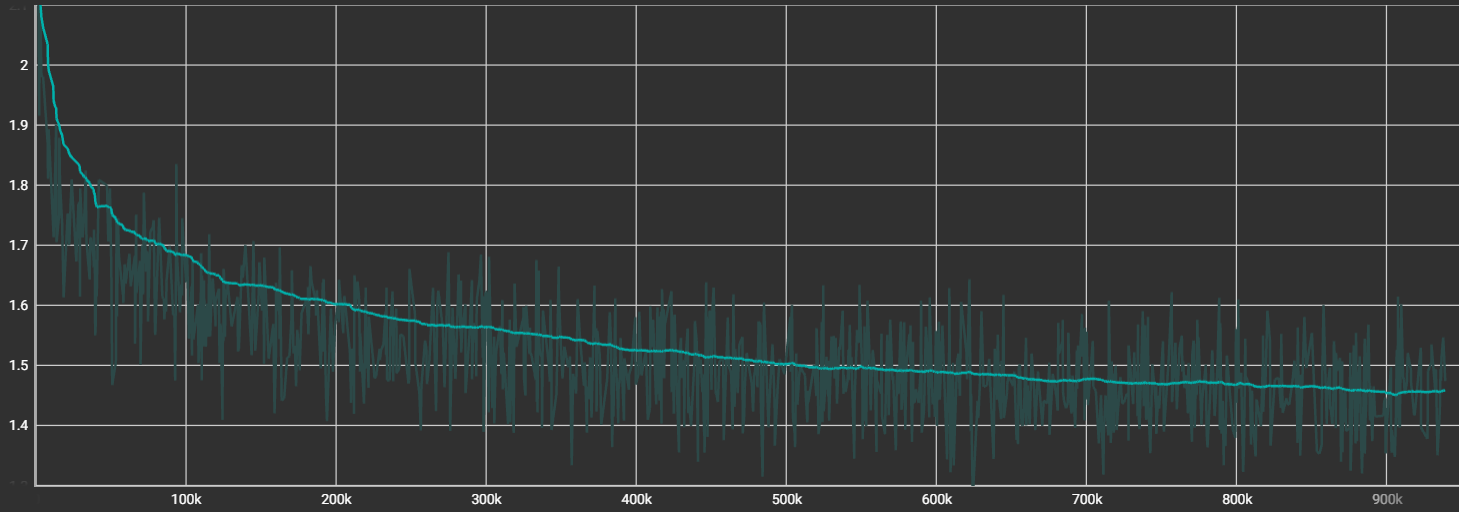
\includegraphics[width=\linewidth]{loss.png}}
\caption{Training loss over time.}
\label{loss figure}
\end{figure}

We evaluated our model on the test set with a size of about 35 thousand positions. We compare the different evaluation functions using the L\textsuperscript{1} distance, also known as Mean Absolute Error (MAE), for the same reason that we used it as the loss function in Section \ref{methodology}. We also take the Root Mean Squared Error (RMSE) into consideration, because it gives equal weight to all errors and penalizes large errors more heavily than small errors. Table \ref{eval table} shows the result of our evaluation.

\begin{table}[htbp]
\caption{Evaluation Results}
\begin{center}
\begin{tabular}{| m{5em} || m{4em} | m{4em} | m{4em} | m{4em} |} \hline
Evaluation Function & Always Zero & Material Count & Piece Square Table & ANN \\ \hline
MAE & 3.94 & 2.47 & 2.39 & 1.47 \\ \hline
RMSE & 6.35 & 4.24 & 4.13 & 2.77 \\ \hline
\end{tabular}
\label{eval table}
\end{center}
\end{table}

The results of this experiment show that our ANN achieved an drastically better performance in both metrics in comparison to the simple evaluation functions. This suggests that our ANN can accurately evaluate chess positions. 


\section{Related work}\label{related work}

In recent years, artificial neural networks (ANNs) have shown great potential in the field of computer chess. Several researchers have explored the use of ANNs to evaluate chess positions and improve the strength of chess engines.

In 2017 Sabatelli et al. \cite{b6} started investigating the strength of Neural Networks for evaluating chess positions. They compared different board representations and model architectures training on 3 million positions. They showed that a representations in bitboards, similar to the way we did, performs better than a saving the piece values of all pieces on a single board.

A new architecture was proposed by Yu Nasu in 2018 for the game Shogi \cite{b7}. It is called Efficiently Updatable Neural Nnetwork (NNUE). In 2019 and 2020 the architecture was successfully ported to chess and integrated into the Stockfish engine. The training process work similar to the one proposed by us with an improved board representation. The neural network is updated using an incremental learning approach, which allows it to adapt to new positions as they are encountered during gameplay.

The use of NNUE has been shown to significantly improve the performance of traditional chess engines. In a recent benchmark test it was revealed that Stockfish NNUE was stronger than the classical one by at least 80 Elo \cite{b8}.

Another interesting approach was introduced in 2017 by Silver et al. when they published their paper about AlphaZero \cite{b9}. AlphaZero is a computer program that uses a combination of deep neural networks and Monte Carlo tree search to play the games of chess, shogi, and Go. AlphaZero is a significant achievement in the field of artificial intelligence and game playing, as it demonstrated that a single algorithm can master multiple complex games without any prior knowledge beyond the rules.

Overall, these advances in the field of game-playing AI have demonstrated the potential of deep learning and reinforcement learning techniques to tackle complex problems in a variety of domains.

\section{Conclusion}\label{conclusion}
In this paper, we presented a method to evaluate chess positions using an Artificial Neural Network (ANN). We trained the ANN on a large data set of positions and achieved a high accuracy in evaluating chess positions.

Our results showed that the ANN was able to outperform traditional evaluation methods, such as the piece square tables, and demonstrated a better understanding of the complex relationships between pieces and their positions on the board.

The ability to quickly and accurately evaluate chess positions can greatly improve the performance of computer chess engines and lead to more engaging and challenging games for human players.

In conclusion, our work highlights the potential of using Artificial Neural Networks to improve the evaluation of chess positions. While our method achieved promising results, there is still room for improvement and further research could explore the use of more advanced neural network architectures and training techniques. 

\section{Supplementary material}\label{supplementary material}

All code used in this paper, including the implementation of the neural network and the preprocessing scripts, is publicly available on GitHub at the following URL: \url{https://github.com/Niklas267/chess-ann}.
The full data set for the training is not in this repository as it has a size of almost 500 GB, but an step-by-step explanation on how to convert the Lichess pgn file can be found. 

The LaTeX file to generate this paper can also be found in the repository.

The code and data sets provided here can be used to reproduce the results reported in this paper, as well as to extend the analysis to new data sets and research questions.

\begin{thebibliography}{00}
\bibitem{b1}“Kasparov-Deep Blue 1997,” www.chessgames.com. \url{https://www.chessgames.com/perl/chesscollection?cid=1030300} (accessed Mar. 15, 2023).

\bibitem{b2}“lichess.org open database,” database.lichess.org. \url{https://database.lichess.org/}

\bibitem{b3}N. Fiekas, “python-chess: a chess library for Python,” GitHub, May 04, 2023. \url{https://github.com/niklasf/python-chess} (accessed May 05, 2023).

\bibitem{b4}“pgn-extract: Portable Game Notation (PGN) Manipulator for Chess Games,” \url{www.cs.kent.ac.uk}. \url{https://www.cs.kent.ac.uk/people/staff/djb/pgn-extract/} (accessed May 05, 2023).
‌
\bibitem{b5}C. E. Shannon, “XXII. Programming a computer for playing chess,” The London, Edinburgh, and Dublin Philosophical Magazine and Journal of Science, vol. 41, no. 314, pp. 256–275, Mar. 1950, doi: \url{https://doi.org/10.1080/14786445008521796}.

\bibitem{b6}M. Sabatelli, F. Bidoia, V. Codreanu, and M. Wiering, “Learning to Evaluate Chess Positions with Deep Neural Networks and Limited Lookahead.” Accessed: Apr. 11, 2023. [Online]. Available: \url{https://www.ai.rug.nl/~mwiering/GROUP/ARTICLES/ICPRAM_CHESS_DNN_2018.pdf}

\bibitem{b7}Y. Nasu “Efficiently Updatable Neural-Network-based Evaluation Functions for Computer Shogi 1,” 2018. Available: \url{https://dev.exherbo.org/~alip/doc/nnue_en.pdf}
‌
‌\bibitem{b8} “Introducing NNUE Evaluation - Stockfish - Open Source Chess Engine,” \url{stockfishchess.org}. \url{https://stockfishchess.org/blog/2020/introducing-nnue-evaluation/}

\bibitem{b9} D. Silver et al., “Mastering Chess and Shogi by Self-Play with a General Reinforcement Learning Algorithm,” Dec. 2017. Available: \url{https://arxiv.org/pdf/1712.01815.pdf}

\end{thebibliography}
\end{document}
